\chapter{Progettare l'Interazione fra Uomo e Macchina}

La rivoluzione tecnologica degli ultimi anni ha portato a parlare molto di User Experience Design, User Interface Design, Interaction Design etc.\\ 

Cosa si intende con il termine \textbf{Design}?\\

Da Treccani.it: \textit{design s. ingl. [propr. «disegno, progetto», dal fr. dessein, che a sua volta è dall’ital. disegno], usato in ital. al masch. – Nella produzione industriale, progettazione (detta più precisamente industrial design) che mira a conciliare i requisiti tecnici, funzionali ed economici degli oggetti prodotti in serie, così che la forma che ne risulta è la sintesi di tale attività progettuale; quando la forma dell’oggetto viene elaborata indipendentemente dalla progettazione vera e propria, si parla più propriam. di styling design. Con riferimento ad altri settori di operatività: graphic d., la ricerca creativa e la progettazione di libri, di stampati pubblicitarî; town d., la progettazione (generalmente a opera di un architetto) mirante a dare ordine e forma a parti di città, ad attrezzature collettive, a parchi pubblici; visual d., la progettazione d’immagini per l’informazione visiva: cartelli, simboli, segnali; web d., l’ideazione e la progettazione di siti Internet.}\\

In Italiano tendiamo quindi ad usare il termine design per riferirci sia al processo di progettazione che al risultato stesso di questo processo:

\begin{flushleft}
    \textit{(processo)``...E' stato avviato il design dell'interfaccia grafica''}\\
    \textit{(risultato del processo)``...Ecco il design dell'interfaccia grafica pronto per essere implementato''}\\
\end{flushleft}


 Per design si intende quindi \textbf{sia il processo di progettazione e pianificazione che l'output stesso di questo processo}. \\
 
 E' importante notare che nel mondo del design, ed in particolare nel design industriale, si approccia alla risoluzione dei problemi e alla progettazione con una forma mentis molto diversa rispetto a quella ``computazionale'' tipica del mondo informatico.
 
 Nel 2006 Jeannette Wing, direttrice del Dipartimento di informatica della Carnegie Mellon University, formulò la seguente definizione di Pensiero Computazionale:
\textit{``il pensiero computazionale è un processo di formulazione di problemi e di soluzioni in una forma che sia eseguibile da un agente che processi informazioni.''}

La stessa Wing ha inoltre messo a fuoco alcune caratteristiche del Computational Thinking: esso non consiste semplicemente nel saper programmare, ma nel pensare a diversi livelli di astrazione; è un’abilità fondamentale per tutti, che dovrebbe diventare la quarta abilità di base oltre al saper ``leggere, scrivere e fare di conto''.

Il pensiero computazionale è quindi un processo mentale che consente di risolvere problemi di varia natura seguendo metodi e strumenti specifici, pianificando una strategia; abitua al rigore e quindi rende possibili gli atti creativi. Permette di interagire con persone e strumenti, di fruire delle potenzialità delle macchine quali oggetti capaci di compensare le lentezze o l’imprecisione dell’uomo, se ben programmati.

Come tutte le scienze, ha i suoi fondamenti formali nel linguaggio matematico e ha a che fare con oggetti del mondo reale. Il pensiero computazionale è infatti basato sulla suddivisione di un problema in sotto-problemi così da poter giungere ad una formalizzazione del problema sotto forma di algoritmo (serie di passi). 

Nel modo del design invece, la progettazione è tipicamente affrontata in maniera globale. L'obbiettivo principale del design di prodotto non è necessariamente quello di trovare una soluzione al problema specifico ma è piuttosto quella di \textbf{comprendere il problema stesso nel suo insieme.}

Nel mondo del design il primo passo è sempre quello di capire perchè il problema esiste e solo dopo aver appurato che l'origine di un problema non può essere eliminata o mitigata ci si adopera per cercare di risolverlo nello specifico. Viceversa, l'informatico medio non appena si trova davanti ad un problema, apre il proprio editor di testo e inizia a scrivere un algoritmo per cercare di risolverlo senza neanche chiedersi se il problema che si sta affrontando esiste veramente.\\

\textit{Cosa vuol dire ``se il problema esiste veramente?''}\\

George Berkeley, un filosofo irlandese del '700 sosteneva che gli oggetti esistono solo in quanto percepiti. Dunque, se un albero cade in una foresta e nessuno lo sente, non fa rumore.

Estesa al mondo dell'interazione uomo-macchina e dello sviluppo prodotto in generale, la filosofia di Berkeley ci dice quindi che se un problema non è percepito da un utente allora quel problema non esiste. Nel design dell'interazione e quindi dell'esperienza utente l'obbiettivo primo è (dovrebbe essere) quindi quello di avere un utente soddisfatto non un software teoricamente perfetto or super-ricco di funzionalità.

 %Si evince quindi che, nel pensiero computazionale si raggiunge un risultato quando si ottiene un algoritmo che è in grado di risolvere il problema dato. Questo problema per poter essere risolto tramite un algoritmo deve essere matematicamente descrivibile e deve avere ingressi, uscite, vincoli e requisiti chiari, definiti e immutabili (nella loro definizione).
 
Questo può portare a situazioni che dal punto di vista informatico sono percepite come assurde. Nel design di prodotto ci si trova infatti spesso costretti a modificare i requirement e le specifiche di prodotto per andare in contro alle esigenze degli utenti e sacrificando funzionalità tecniche e qualità dell'implementazione software.
 Trovare il corretto bilanciamento fra esperienza utente, funzionalità e qualità tecnica è la parte più complessa dell'intero processo di sviluppo prodotto. Nei prossimi capitoli introdurremo delle tecniche e dei processi atti a gestire questo processo in maniera scientifica e strutturata.
 
 %e cioè assurda (dal punto di vista informatico) condizione in cui si modificano gli obbiettivi dello sviluppo al fine di assolvere alle esigenze dell'utente in termini di esperienza.
 
Questo processo antropocentrico di adattamento del software alle esigenze dell'utente piuttosto che al virtuosismo tecnico è spesso vissuto dalla maggior parte degli informatici come un'assurda violenza. Per questo motivo è molto importante che gli informatici studino i principi del design, perchè il mondo del design antropocentrico è per i tecnici tipicamente molto molto complicato da metabolizzare in quanto distante dal pensiero computazionale.

E' importante evidenziare che design dell'interazione e pensiero computazionale non sono mutualmente esclusivi, anzi. E' nell'unione dei due e nell'integrazione dei due processi di studio e progettazione che nascono prodotti di successo e software di qualità. \\

%Ogni cosa con cui abbiamo quotidianamente a che fare è il risultato di un processo di design; una lampada, una strada, una casa. Nella progettazione di oggetti interattivi e interfacce utente però non possiamo limitarci alla progettazione puramente estetica. E' necessario infatti andare oltre l'aspetto fisico e la piacevolezza alla vista o al tatto di un oggetto e curarci dell'esperienza e quindi della sensazione che l'utente proverà nell'interagire con l'oggetto (frutto) del nostro design. Un'interfaccia molto bella e graficamente accattivante ma impossibile da utilizzare è sicuramente un pessimo risultato per un processo di design.

\begin{flushleft}
\textbf{ \textit{``If we want users to like our software, we should design it to behave like a likeable person: respectful, generous and helpful.''}}\\

\textit{Alan Cooper, software designer e programmatore, noto come "il padre del Visual Basic"}
    
\end{flushleft}


\section{Interaction Design}
Il mondo della progettazione è diventato talmente ampio e variegato che il termine design da solo ormai non ha quasi più significato. Esistono varie sotto discipline del design e con queste numerose professioni, metodi di lavoro, scuole di pensiero e altrettante immancabili faide e lotte fra fazioni.

Un informatico può fare a meno di conoscere al completo il mondo del design ma non può esimersi da possedere i rudimenti base del ``design dell'interazione''.

Interaction design, o progettazione dell'interazione, è l'attività di progettazione dell'interazione che avviene tra esseri umani e oggetti in generale. 

%e la fruizione di servizi e sistemi complessi in modo proficuo e soddisfacente.

L'obiettivo principale dell'interaction design è quello di rendere macchine, servizi e sistemi usabili dagli utenti per cui sono stati pensati e realizzati e non solamente dai propri creatori. All'interno di un processo di interaction design, si investigano l'uso che verrà fatto dell'artefatto e il target a cui esso si rivolge. Questo significa che le questioni legate agli utenti guidano il processo più di quanto non facciano le questioni tecniche. Gli sviluppatori devono mettere al centro del processo di sviluppo i bisogni degli utenti, arrivando a realizzare un prodotto più appropriato e maggiormente usabile. Le forze trainanti lo sviluppo di un prodotto dovrebbero essere quindi gli utenti reali e i loro bisogni e non solo le tecnologie.


%Uno dei principali e normalmente più visibili campi di intervento è la progettazione delle interfacce, attraverso cui avviene l'interazione uomo-macchina.

Nel nostro caso ci focalizzeremo sull'interazione fra uomo e sistemi informatici e quindi andremo a lavorare nel campo dell'interazione uomo-macchina e uomo-computer (in Inglese HMI Human-Machine Interaction e HCI Human Computer Interaction). L'obbiettivo principale del HMI e HCI design è quindi rendere possibile e facilitare al massimo, per un essere umano, l'uso e l'interazione con sistemi del mondo IT (Information Technology) quali, calcolatori, dispositivi mobili, servizi web etc.

Interaction design, HMI e HCI sono discipline molto variegate ed ampie che spaziano dall'informatica, alla psicologia, passando per la grafica e l'ingegneria. 

Capiamo meglio il mondo dell'Interaction design analizzando in dettaglio alcune sotto discipline del design: il \textbf{design di prodotto}, il \textbf{design dell'esperienza utente} e il \textbf{design dell'interfaccia}. 


\begin{figure}[!h]
	\centering
	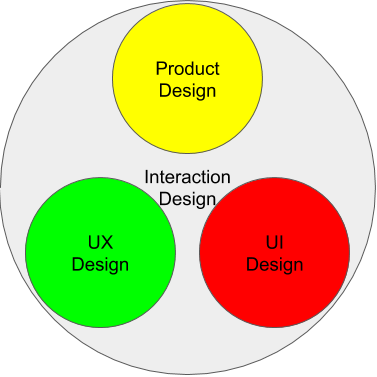
\includegraphics[width=0.8\textwidth]{immagini/interactiondesign2.png}
	\caption{Il design dell'interazione è un un settore altamente interdisciplinare in cui si vanno a compenetrare diverse discipline.}
\end{figure}

Prima di entrare nel dettaglio è importante sottolineare che nessuna di queste discipline o settori della progettazione è rigidamente definite e spesso le tre si intrecciano e vengono quindi eseguite da team multi disciplinari. Inoltre, specialmente in piccole aziende e piccoli team di sviluppo non si riesce a separare queste attività di progettazione e quindi è estremamente importante che l'informatico moderno conosca i rudimenti di base necessari per poter contribuire ad un team in cui vengono portate avanti anche questa tipologia di attività.


\subsection{Product Design}
Il \textbf{design di prodotto} è un processo strategico di risoluzione dei problemi che guida l'innovazione e porta a una migliore qualità della vita attraverso prodotti, sistemi, servizi ed esperienze innovative \textit{(definizione ufficiale di disegno industriale, coniata nel 2015 dalla World Design Organization (ex ICSID). Spesso design di prodotto e design industriale sono utilizzati in modo intercambiabile}. 

Nel design di prodotto si progettano quindi beni e servizi il cui obbiettivo principale è quello di essere utilizzati da quanti più utenti possibili migliorandone la vita. Il designer di prodotto è quindi colui che inventa un nuovo modo o un nuovo oggetto per fare cose che fino a ieri non si potevano fare o si facevano in maniera più complicata.

Il design di prodotto è quindi il punto di partenza dei processi di innovazione e rappresenta quindi il punto di partenza del percorso di design dell'interazione che stiamo esplorando.

L'inventore (designer) del prodotto si focalizza su un problema da risolvere e inventa un prodotto che grazie alle sue caratteristiche tecniche permette di risolvere il problema.

Descriviamo un prodotto noto come se stessimo provando a formalizzare un processo di product design atto a reinventare un processo noto e consolidato, ascoltare musica. 

\begin{flushleft}
\textbf{Nome prodotto:} Spotify;\\
\textbf{Problema a cui assolve:} Ascoltare musica senza possederla;\\
\textbf{Tipologia di prodotto:} Servizio basato su Internet;\\
\textbf{Funzionalità principale:} Consentire l'ascolto di qualunque brano, su qualsiasi piattaforma senza richiedere l'acquisto di un supporto fisico e dei diritti d'autore;\\
\textbf{Soluzioni esistenti:} Noleggio/prestito CD e altri supporti fisici, download di musica pirata;
\textbf{Soluzione:} Servizio di streaming basato su business model "freemium" che di fatto rappresenta un jukebox con brani pressoché illimitati;
\textbf{Requisiti per l'utilizzo:} PC o smartphone o tablet, Connessione internet. 
\end{flushleft}

Estremizzando un po' i concetti potremmo dire che il product designer di Spotify ha terminato il suo lavoro. Quello sopra descritto è il frutto del processo di design di prodotto che ha portato alla nascita di un servizio rivoluzionario come Spotify. Non c'è tanto altro da aggiungere per descrivere il concetto che sta alla base del prodotto e quindi l'innovazione che esso introduce.

\begin{figure}[!h]
	\centering
	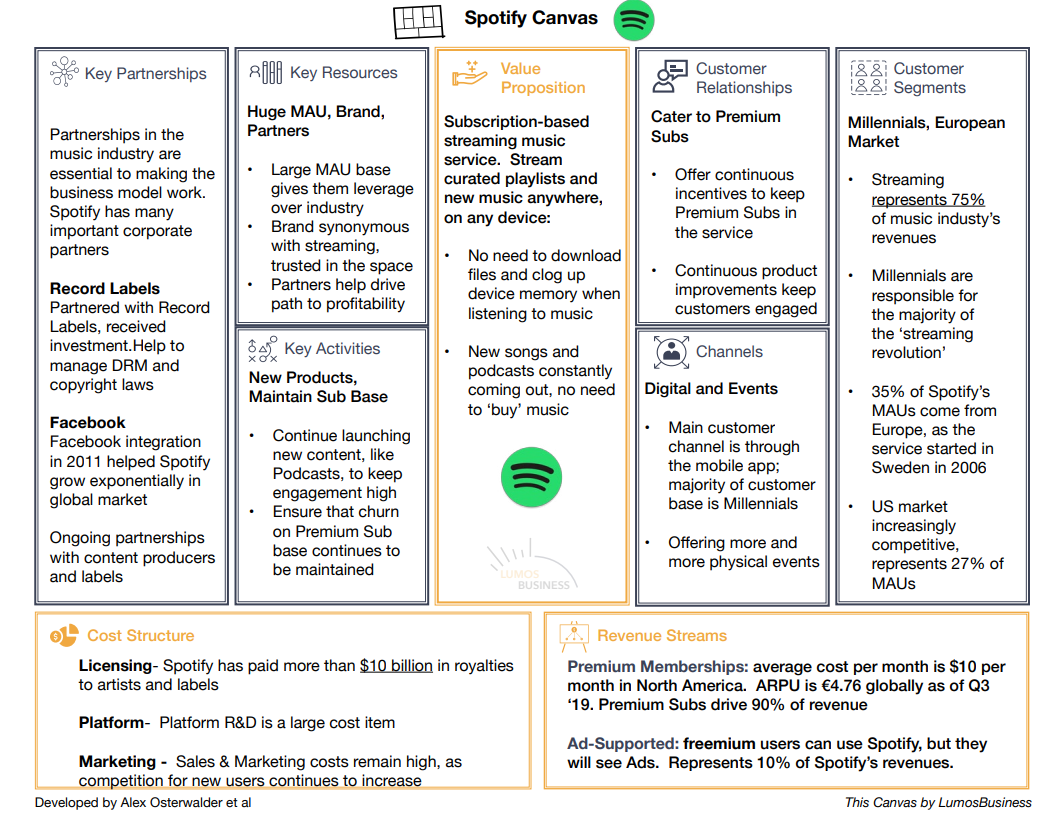
\includegraphics[width=\textwidth]{immagini/spotifycanvas.png}
	\caption{Business model canvas di Spotify. Fonte http://lumosbusiness.com/business-model-canvas-spotify/}
\end{figure}

E' chiaro però che questo nuovo prodotto potrebbe essere realizzato in tanti modi e che sarà proprio il modo in cui viene costruito a decretarne il successo o il fallimento del prodotto. Questo perchè non basta un'idea per fare un prodotto di successo, ci vuole un lungo e complicato processo di progettazione che vada oltre l'idea e metta al centro l'utente, i suo bisogni e le sue aspettative.

\subsection{User Experience Design}
Il \textbf{design dell'esperienza utente} è il processo volto ad aumentare la soddisfazione e la fedeltà del cliente migliorando l'usabilità, la facilità d'uso e il piacere fornito nell'interazione tra il cliente e il prodotto. La progettazione dell'esperienza utente comprende la tradizionale progettazione dell'interazione uomo-macchina e la estende integrandola con tutti gli aspetti di business, marketing e sviluppo prodotto necessari per garantire il successo del prodotto e/o servizio.

%L'esperienza utente è qualsiasi aspetto di un'interazione della persona con un dato sistema informatico e interattivo. La progettazione dell'esperienza studia il prodotto nel suo insieme trattando aspetti legati all'interfaccia, alla grafica, alla progettazione industriale e all'interazione fisica e manuale.

Ogni prodotto durante l'utilizzo da parte di un utente porta a far vivere un esperienza e di conseguenza si dice abbia una sua ``user experience''. Ovviamente, la user experience non è una proprietà del prodotto in se ma piuttosto una relazione che intercorre fra il prodotto ed uno specifico utente. Il tema delle relazioni e della relatività delle esperienze verrà meglio affrontato nei capitoli successivi. 

%Per ora limitiamoci a sottolineare che non è possibile progettare l'esperienza utente ma si progetta \textbf{per} l'esperienza utente.

Lo \textbf{UX Designer} ha quindi l'obbiettivo di far vivere all'utente del suo prodotto la miglior esperienza possibile, evitando quindi che l'oggetto induca nell'utente sensazioni di frustrazione e delusione.
Spesso si tende a dire che si ``progetta l'esperienza utente''. In realtà è impossibile progettare l'esperienza utente perchè ogni utente è diverso dall'altro ed è quindi illusorio pensare che chiunque durante l'utilizzo del prodotto si comporti alla stessa maniera e in particolare si comporti esattamente come il progettista ha ipotizzato.
E' quindi corretto dire che si ``progetta \textbf{per} l'esperienza utente''.

Come vedremo nei capitoli successivi, lo studio e la progettazione dell'esperienza utente partono sempre dalla analisi e comprensione delle esigenze dell'utente e non dalle specifiche funzionali di prodotto. 

\subsection{User Interaction Design}
Il Design dell'interazione ha come focus il modo in cui le persone interagiscono con la tecnologia, lo scopo è migliorare la loro comprensione di ciò che si può fare, ciò che succede e ciò che è appena successo, basandosi su principi psicologici, tecnici ed estetici.

Dallo studio della UX si crea quindi uno schema di interazione che poi viene passato allo \textbf{UI Designer} che ha il compito di progettare l'interfaccia utente al fine di abilitare l'esperienza progettata.
%un abbozzo dell'interfaccia. Non si crea subito il \textit{wireframe} finale, bensì si parte da un'analisi dei casi di studio. Esistono più tipi di casi di studio ed ognuno è specifico per delle personas, infatti, personas differenti hanno capacità differenti.

Lo UI designer non costruisce quindi l'interfaccia utente, nei team numerosi questa figura è spesso un progettista grafico e non un informatico. L'obbiettivo dello UI designer è quello di progettare l'aspetto estetico e la struttura dell'interfaccia così che questa durante l'utilizzo induca l'utente nel seguire l'esperienza che è stata per lui progettata.
Lo UI designer produce quindi un wireframe, una bozza grafica, dell'interfaccia e una serie di linee guida che poi veranno seguite dagli sviluppatori (UI developer o Front-end developer) per implementare la reale interfaccia del prodotto o servizio

\begin{figure}[!h]
	\centering
	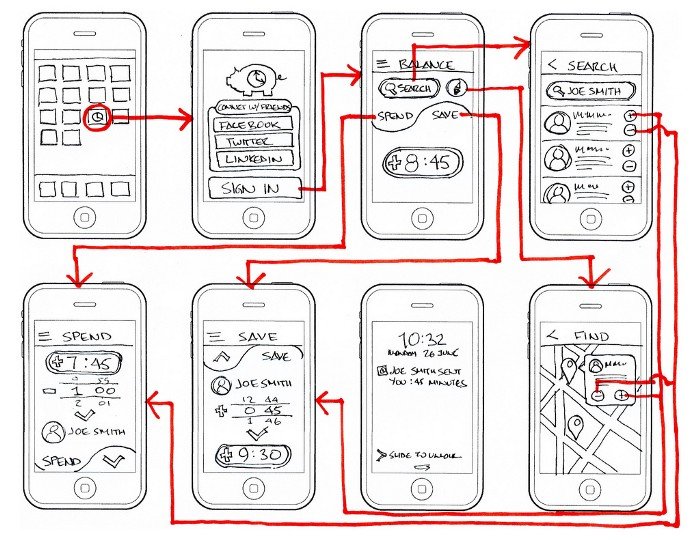
\includegraphics[width=\textwidth]{immagini/uidesign.jpeg}
	\caption{Esempio di progetto di UI per una App mobile. Il wireframe riporta le linee guida per la struttura dell'interfaccia e il flusso utente (implementato a partire dal lavoro di UX Design). Fonte: https://blog.prototypr.io/why-you-shouldnt-skip-your-wireframing-1f7a70d5c125}
\end{figure}

%o differente dal front-end developing: la materia progetta le guidelines che istruiscono il developer su come creare al meglio una UI.

%Non è sbagliato considerare lo UI Design come \textbf{sotto area} dello UX Desing.

Il processo di Product Design è quindi un percorso strutturato che include varie figure e discipline. In grandi team questi step sono eseguiti tipicamente da diverse persone e team ma spesso nella media e piccola impresa o startup questo percorso deve poter essere seguito in autonomia da una o al massimo due figure.

L'interfaccia vera e propria viene implementata quindi solo alla fine del percorso di progettazione da figure con profilo tecnico informatico (Front End Developer o UI Developer). Queste figure devono quindi essere in grado di comprendere le richieste provenienti dagli step di progettazione precedenti e quindi devono possedere i rudimenti base dell'Interaction Design e delle relative sotto discipline.

\begin{figure}[!h]
	\centering
	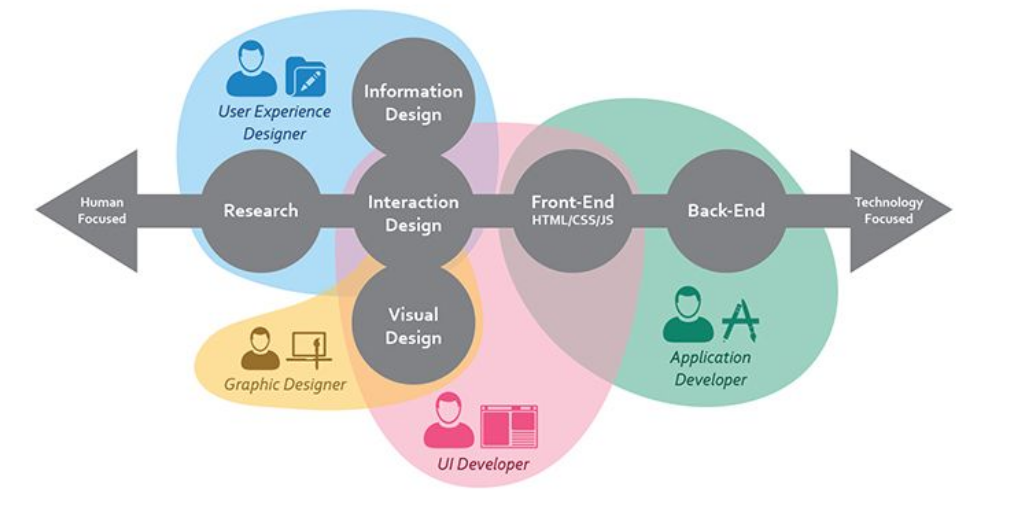
\includegraphics[width=\textwidth]{immagini/UX_and_UI.png}
	\caption{Flusso di lavoro e ruoli necessari per lo sviluppo di un prodotto. fonte: https://www.crayondata.com/blog/the-difference-between-ui-and-ux/
}
\end{figure}

